En Argentina el 95\% de los incendios forestales se derivan de actividades humanas\cite{ministerio_2021}. La sequía, el nivel más bajo del río en los últimos 50 años y el uso del fuego para eliminar los pastos nativos\cite{borus_2020}, provocaron cifras récord de incendios en el año 2020 en el Delta del río Paraná. Actualmente los incendios en las islas del río Paraná, son captados satelitalmente (a una dada hora del día) o por alcance del humo a las zonas habitadas. En este reporte se presenta un análisis de los incendios en el humedal frente al cordón poblacional de Villa Constitución - San Nicolás, ocurridos entre el 10 y el 16 de junio 2021.\\

Para el conteo de los focos de incendios se utilizaron los datos de la plataforma de Información sobre Incendios para el Sistema de Gestión de Recursos (FIRMS, por sus siglas en inglés), propiedad de la NASA (Administración Nacional de Aeronáutica y el Espacio, de los Estados Unidos de América). En particular, se procesaron los datos de los incendios detectados por el instrumento satelital VIIRS-Suomi NPP, el cual pasa por la región del Delta del río Paraná entre las 13:00 - 16:00 hora local.\\

Con un programa propio se contabilizaron los focos de incendios sólo en el área del humedal (Figura \ref{fig:conteo}). Se delimitó esta zona a fin de excluir los puntos sobre las ciudades de Villa Constitución y San Nicolás, que con frecuencia son señalados como focos incendios debido a la alta temperatura generada por la actividad industrial. El mayor número de incendios sobre el Delta fueron detectados los días 12, 13 y 14 con el instrumento VIIRS-Suomi. Debido a la larga duración de los incendios también fueron detectados por los instrumentos satelitales MODIS y VIIRS-NOAA que pasan a otra dada hora del día.

\begin{figure}[H]
    \centering
    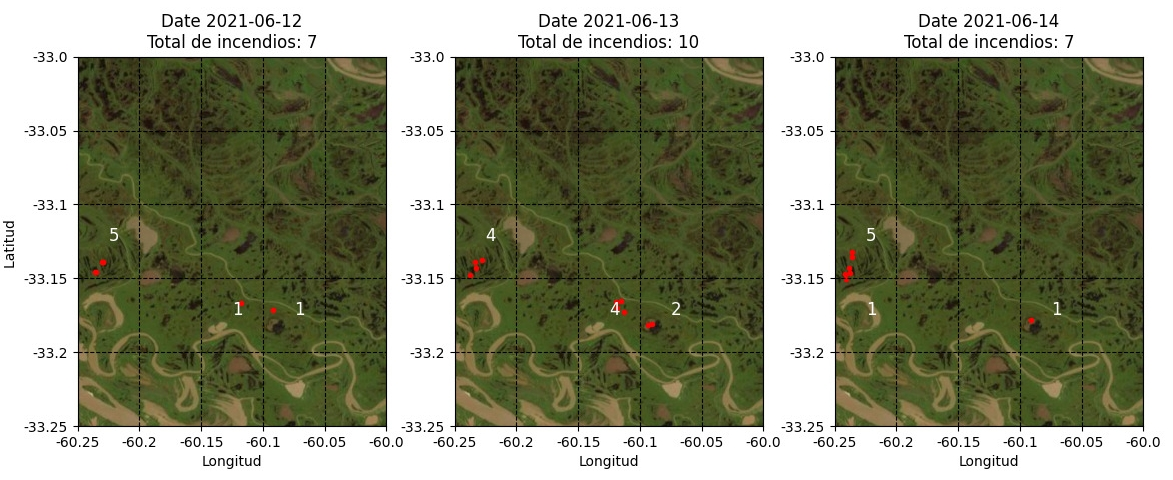
\includegraphics[width=0.8\paperwidth]{images/image2.jpg}
    \caption{Localización geográfica y número de focos de incendios en el humedal del río Paraná, frente al cordón poblacional de Villa Constitución-San Nicolás, los días: 12, 13 y 14 de junio 2021.}
    \label{fig:conteo}
\end{figure}

En ausencia de instrumentos in situ para medir la contaminación atmosférica durante los incendios, se tomaron los datos del Servicio de Monitoreo de la Atmósfera Copernicus (CAMS, por sus siglas en inglés) del Centro Europeo de Previsiones Meteorológicas a Plazo Medio. Los datos derivados del CAMS de material particulado de tamaño menor o igual a 10 micrones (PM\textsubscript{10}) y de tamaño menor o igual a 2.5 micrones (PM\textsubscript{2.5}), así como de la velocidad y dirección del viento, se muestran en la Tabla \ref{table:numero_de_incendios}. En particular, los valores de PM10 y PM2.5 representan una concentración a gran escala y no mediciones a nivel del suelo. El día 13 de junio, el viento del Norte arrastró el humo y los aerosoles hacia las zonas habitadas. El sistema del CAMS para ese día mostró un valor de PM\textsubscript{2.5} de 9$\mu$gr/m\textsuperscript{3}, mientras que en una región no afectada (opuesta a la dirección del viento), mostró un valor de 4$\mu$gr/m\textsuperscript{3}. Durante los 7 días los valores de PM\textsubscript{2.5} fueron en promedio un 58\% más altos que aquellos estimados en las regiones no afectadas por el humo.

\begin{table}[H]
    \centering
    \begin{tabular}{llllll}
        \hline
        Fecha 2021              & \begin{tabular}[c]{@{}l@{}}Incendios\\ diarios\end{tabular} & \begin{tabular}[c]{@{}l@{}}Incendios\\ acumulados\end{tabular} & \begin{tabular}[c]{@{}l@{}}*PM2.5 \\ ($\mu$gr/m\textsuperscript{3})\end{tabular} & \begin{tabular}[c]{@{}l@{}}*PM10\\  ($\mu$gr/m\textsuperscript{3})\end{tabular} & \begin{tabular}[c]{@{}l@{}}*Velocidad  (km/h) \\ y Dirección del viento\end{tabular} \\ \hline
        \multirow{2}{*}{10/Jun} & 2                         & 2                         & 13                        & 19                        & 12 SSO                    \\
                                & 6                         & 8                         & 3                         & 5                         & 11 NO                     \\
        \multirow{4}{*}{12/Jun} & 7                         & 15                        & 10                        & 14                        & 12 N                      \\
                                & 10                        & 25                        & 9                         & 14                        & 15 N                      \\
                                & 7                         & 32                        & 16                        & 24                        & 11 S                      \\
                                & 2                         & 34                        & 16                        & 22                        & 8 SSE                     \\
        16/Jun                  & 2                         & 36                        & 19                        & 28                        & 5 SSE                     \\ \hline
    \end{tabular}
    \caption{Fecha, número de focos de incendio diario y acumulado, PM\textsubscript{2.5} , PM\textsubscript{10} y velocidad y dirección del viento. (*) Valores del CAMS a las 15:00h en la región del humedal del río Paraná. El PM\textsubscript{10} y PM\textsubscript{2.5} son una referencia a gran escala y no representan la contaminación del aire a nivel local.}
    \label{table:numero_de_incendios}
\end{table}

La quema de biomasa y el viento en dirección Norte pueden contribuir significativamente a la mala calidad del aire de las ciudades localizadas a la orilla del río Paraná. Por otro lado, el día 14, el viento del Sur dirigió el humo en sentido contrario a la zona habitada (Figura \ref{fig:FIRMS}).

\begin{figure}[H]
    \centering
    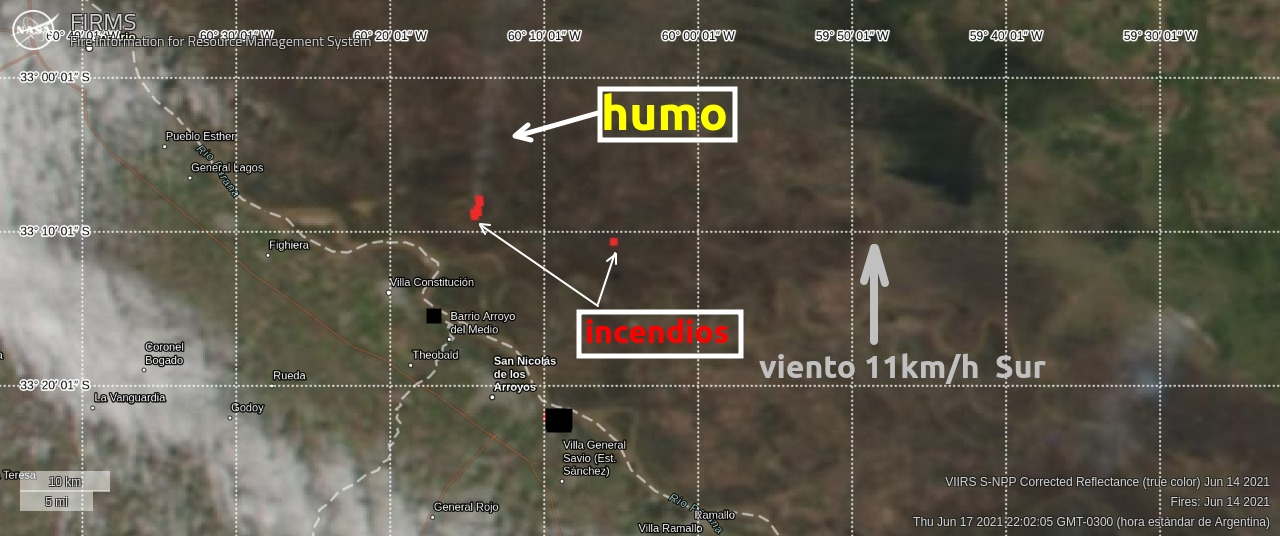
\includegraphics[width=0.8\paperwidth]{images/image1.jpg}
    \caption{Imagen del FIRMS el día 14 de junio 2021 frente al cordón Villa Constitución-San Nicolás.}
    \label{fig:FIRMS}
\end{figure}

Para una alerta temprana de incendios y medición de la calidad del aire in situ, se recomienda adquisición de instrumentos de material particulado.